\section{Технический проект}
\subsection{Общая характеристика организации решения задачи}

Необходимо спроектировать и разработать базу данных для корпоративного мессенджера, которая должна обеспечивать надежное хранение и быстрый доступ к сообщениям, пользовательским данным и информации о группах.

База данных представляет собой структурированный набор взаимосвязанных таблиц, содержащих текстовую информацию (сообщения, имена пользователей), метаданные (временные отметки, идентификаторы) и системные данные (роли, статусы). База располагается в файле data.db и использует SQLite в качестве системы управления.

\subsection{Обоснование выбора технологии проектирования}

Для реализации корпоративного мессенджера рассмотрены различные СУБД, включая PostgreSQL, MySQL и SQLite. Выбор SQLite обусловлен следующими факторами:

\subsubsection{Система управления базами данных SQLite}

SQLite — встраиваемая реляционная СУБД, не требующая отдельного серверного процесса. Основные преимущества в контексте проекта:

\begin{itemize}
	\item нулевая конфигурация — не требует администрирования;
	\item компактность — вся база в одном файле;
	\item высокая производительность для операций чтения/запись;
	\item полная поддержка транзакций ACID.
\end{itemize}

\subsubsection{Достоинства SQLite для данного проекта}
\begin{itemize}
	\item идеально подходит для приложений с одним пользователем или небольших рабочих групп;
	\item не требует отдельного сервера БД, что упрощает развертывание;
	\item поддерживает большинство возможностей SQL-92.
\end{itemize}

\subsubsection{Ограничения SQLite}
\begin{itemize}
	\item ограниченная поддержка одновременных записей (write-ahead logging включен);
	\item максимальный размер базы данных около 140 TB (достаточно для корпоративного мессенджера);
	\item отсутствие встроенной системы аутентификации пользователей.
\end{itemize}

\subsection{Проектирование модели данных}

Схема базы данных представляет собой визуализацию структуры и взаимосвязей основных модулей системы хранения данных.

\begin{figure}[ht]
\center{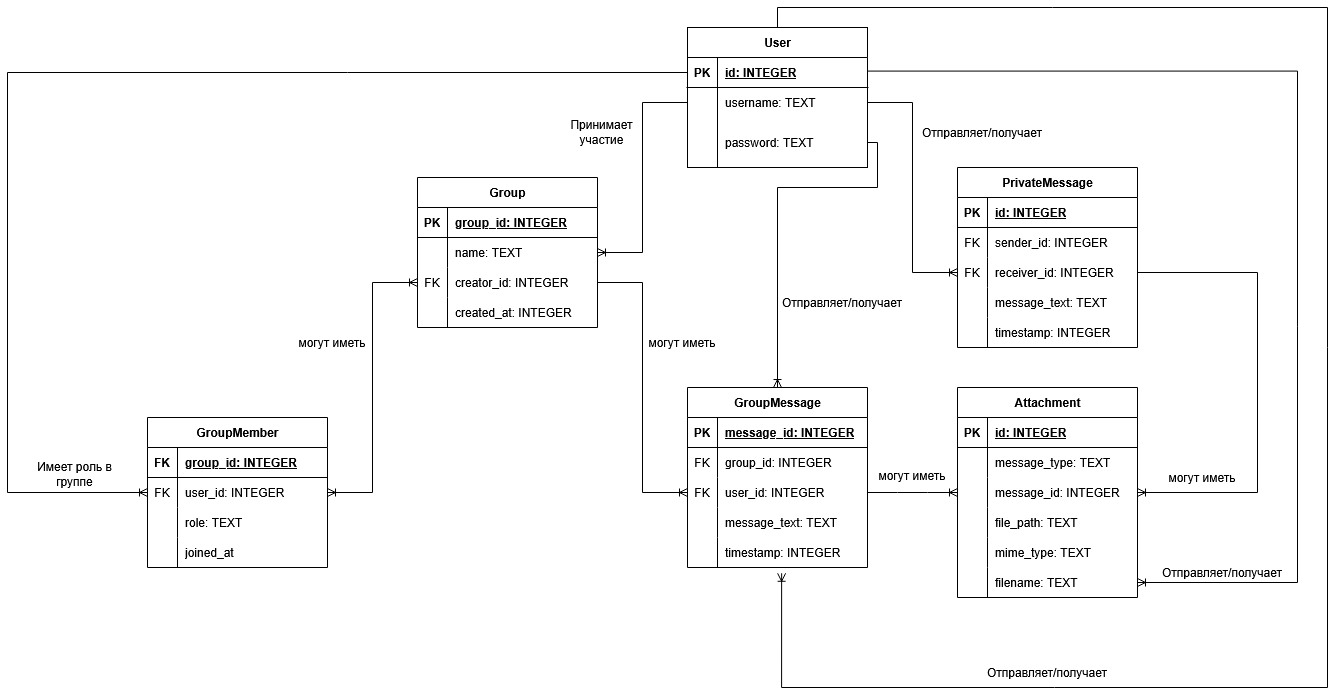
\includegraphics[width=1\linewidth]{ЕР модель}}
\caption{Схема базы данных}
\label{comp:image}
\end{figure}

ER-модель отражает строгую структуру данных, построенную вокруг взаимодействия пользователей в групповых и приватных чатах. В центре системы находится сущность "Пользователь", хранящая учетные данные и выступающая отправителем сообщений. Группы организуют коллективное общение, фиксируя создателя и время создания, а Сообщения делятся на групповые и приватные, с обязательной привязкой к отправителю и временной меткой.

Система ролей реализована через связующую сущность "GroupMember", которая определяет права участников групп (владелец, администратор, участник) и дату их присоединения. Это обеспечивает гибкое управление доступом внутри чатов. Для работы с файлами используется сущность "Attachment", привязанная к сообщениям и содержащая технические данные о файлах (путь, тип, оригинальное имя), что позволяет единообразно обрабатывать вложения как в групповых, так и в личных сообщениях.

Модель подчеркивает важность целостности данных через систему внешних ключей, гарантируя, что сообщения не могут существовать без отправителя или чата. Поле "timestamp" обеспечивает учет активности пользователей, а минималистичная реализация приватных чатов (прямая связь отправитель-получатель) упрощает архитектуру. Вынос вложений в отдельную таблицу позволяет менять способ хранения файлов без изменения структуры сообщений.

\subsection{Таблицы базы данных}
\subsubsection{User - Пользователи системы}
\begin{xltabular}{\textwidth}{|l|l|X|}
	\caption{Атрибуты сущности "Пользователи"\label{user:table}}\\ \hline
	\centrow Поле & \centrow Тип & \centrow Описание \\ \hline
	\thead{id} & \thead{INTEGER} & Первичный ключ (PK), уникальный идентификатор пользователя \\ \hline
	\thead{username} & \thead{TEXT} & Имя пользователя (уникальное) \\ \hline
	\thead{password} & \thead{TEXT} & Хэшированный пароль пользователя \\ \hline
\end{xltabular}

Таблица "User" хранит информацию о зарегистрированных пользователях мессенджера. Каждый пользователь имеет уникальный идентификатор, имя пользователя и пароль. Является центральной сущностью системы, с которой связаны все остальные таблицы.

\subsubsection{Group - Групповые чаты}
\begin{xltabular}{\textwidth}{|l|l|X|}
	\caption{Атрибуты сущности "Групповые чаты"\label{group:table}}\\ \hline
	\centrow Поле & \centrow Тип & \centrow Описание \\ \hline
	\thead{group\_id} & \thead{INTEGER} & Первичный ключ (PK), ID группы \\ \hline
	\thead{name} & \thead{TEXT} & Название группы \\ \hline
	\thead{creator\_id} & \thead{INTEGER} & Внешний ключ (FK→User), ID создателя группы \\ \hline
	\thead{created\_at} & \thead{INTEGER} & Timestamp создания группы \\ \hline
\end{xltabular}

Таблица "Group" содержит информацию о групповых чатах. Каждая группа имеет уникальный идентификатор, название, создателя и время создания. Создатель группы автоматически становится владельцем (owner).

\subsubsection{GroupMember - Участники групп с ролями}
\begin{xltabular}{\textwidth}{|l|l|X|}
	\caption{Атрибуты сущности "Участники групп"\label{groupmember:table}}\\ \hline
	\centrow Поле & \centrow Тип & \centrow Описание \\ \hline
	\thead{group\_id} & \thead{INTEGER} & Внешний ключ (FK→Group), ID группы \\ \hline
	\thead{user\_id} & \thead{INTEGER} & Внешний ключ (FK→User), ID пользователя \\ \hline
	\thead{role} & \thead{TEXT} & Роль в группе: 'owner' (владелец), 'admin' (администратор), 'member' (участник) \\ \hline
	\thead{joined\_at} & \thead{INTEGER} & Timestamp вступления пользователя в группу \\ \hline
\end{xltabular}

Таблица "GroupMember" определяет состав участников групп и их роли. Реализует систему прав доступа, аналогичную Telegram, где владелец имеет максимальные права, администраторы - ограниченные права управления, а участники - базовые права.

\subsubsection{GroupMessage - Сообщения в группах}
\begin{xltabular}{\textwidth}{|l|l|X|}
	\caption{Атрибуты сущности "Групповые сообщения"\label{groupmessage:table}}\\ \hline
	\centrow Поле & \centrow Тип & \centrow Описание \\ \hline
	\thead{message\_id} & \thead{INTEGER} & Первичный ключ (PK), ID сообщения \\ \hline
	\thead{group\_id} & \thead{INTEGER} & Внешний ключ (FK→Group), ID группы \\ \hline
	\thead{user\_id} & \thead{INTEGER} & Внешний ключ (FK→User), ID отправителя \\ \hline
	\thead{message\_text} & \thead{TEXT} & Текст сообщения (может быть пустым для сообщений с вложениями) \\ \hline
	\thead{timestamp} & \thead{INTEGER} & Время отправки сообщения (timestamp) \\ \hline
\end{xltabular}

Таблица "GroupMessage" хранит все сообщения, отправленные в групповых чатах. Каждое сообщение связано с группой и пользователем-отправителем. Поддерживает текстовые сообщения и сообщения с вложениями (через таблицу Attachment).

\subsubsection{PrivateMessage - Личные сообщения}
\begin{xltabular}{\textwidth}{|l|l|X|}
	\caption{Атрибуты сущности "Личные сообщения"\label{privatemessage:table}}\\ \hline
	\centrow Поле & \centrow Тип & \centrow Описание \\hline
	\thead{id} & \thead{INTEGER} & Первичный ключ (PK), уникальный идентификатор сообщения \\ \hline
	\thead{sender\_id} & \thead{INTEGER} & Внешний ключ (FK→User), ID отправителя сообщения \\ \hline
	\thead{receiver\_id} & \thead{INTEGER} & Внешний ключ (FK→User), ID получателя сообщения \\ \hline
	\thead{message\_text} & \thead{TEXT} & Текст сообщения (может быть пустым для сообщений с вложениями) \\ \hline
	\thead{timestamp} & \thead{INTEGER} & Время отправки сообщения (timestamp) \\ \hline
\end{xltabular}

Таблица "PrivateMessage" хранит историю приватных сообщений между пользователями. Каждое сообщение связывает отправителя и получателя, поддерживает текстовый контент и вложения (через таблицу Attachment). Реализует функционал личной переписки между сотрудниками организации.

\subsubsection{Attachment - Вложения к сообщениям}
\begin{xltabular}{\textwidth}{|l|l|X|}
	\caption{Атрибуты сущности "Вложения"\label{attachment:table}}\\ \hline
	\centrow Поле & \centrow Тип & \centrow Описание \\ \hline
	\thead{id} & \thead{INTEGER} & Первичный ключ (PK), уникальный идентификатор вложения \\ \hline
	\thead{message\_type} & \thead{TEXT} & Тип сообщения: 'general' (системные), 'group' (групповые), 'private' (личные) \\ \hline
	\thead{message\_id} & \thead{INTEGER} & ID сообщения, к которому относится вложение \\ \hline
	\thead{file\_path} & \thead{TEXT} & Путь к файлу в файловом хранилище системы \\ \hline
	\thead{mime\_type} & \thead{TEXT} & MIME-тип файла для корректной обработки клиентом \\ \hline
	\thead{filename} & \thead{TEXT} & Оригинальное имя файла для отображения пользователю \\ \hline
\end{xltabular}

Таблица "Attachment" обеспечивает хранение файловых вложений для всех типов сообщений в системе. Универсальная структура позволяет прикреплять файлы к групповым чатам, личным сообщениям и системным уведомлениям. Содержит метаданные файлов для правильного отображения в клиентских приложениях.

\subsection{Нормализация модели данных}

Нормализация базы данных — это процесс организации данных, направленный на уменьшение избыточности, предотвращение аномалий и повышение целостности системы. Основная цель нормализации заключается в минимизации повторяющихся данных и обеспечении логической структуры хранения. 

В ходе нормализации используются три основные нормальные формы:
\begin{enumerate}
	\item Первая нормальная форма (1NF) — исключает повторяющиеся группы и требует атомарности данных;
	\item Вторая нормальная форма (2NF) — обеспечивает зависимость всех атрибутов от полного первичного ключа;
	\item Третья нормальная форма (3NF) — устраняет транзитивные зависимости, исключая зависимость одного неключевого поля от другого.
\end{enumerate}

\subsubsection{Первая нормальная форма (1NF)}

Первая нормальная форма требует, чтобы все атрибуты таблиц имели атомарные значения, а каждая запись была уникальной. В корпоративном мессенджере эта концепция реализована следующим образом:

\textbf{Таблица User}  
\begin{itemize}
	\item id — уникальный идентификатор, одно значение;
	\item username — имя пользователя, одно значение;
	\item password — хэшированный пароль, одно значение.
\end{itemize}

\textbf{Таблица Group}  
\begin{itemize}
	\item group\_id — уникальный идентификатор группы, одно значение;
	\item name — название группы, одно значение;
	\item creator\_id — идентификатор создателя группы, одно значение;
	\item created\_at — временная метка создания, одно значение.
\end{itemize}

\textbf{Таблица GroupMember}  
\begin{itemize}
	\item group\_id — идентификатор группы, одно значение;
	\item user\_id — идентификатор пользователя, одно значение;
	\item role — роль пользователя в группе (owner, admin, member), одно значение;
	\item joined\_at — временная метка вступления, одно значение.
\end{itemize}

\textbf{Таблица GroupMessage}  
\begin{itemize}
	\item message\_id — уникальный идентификатор сообщения, одно значение;
	\item group\_id — идентификатор группы, одно значение;
	\item user\_id — идентификатор отправителя, одно значение;
	\item message\_text — текст сообщения, одно значение;
	\item timestamp — временная метка отправки, одно значение.
\end{itemize}

\textbf{Таблица PrivateMessage}  
\begin{itemize}
	\item id — уникальный идентификатор, одно значение;
	\item sender\_id — идентификатор отправителя, одно значение;
	\item receiver\_id — идентификатор получателя, одно значение;
	\item message\_text — текст сообщения, одно значение;
	\item timestamp — временная метка отправки, одно значение.
\end{itemize}

\textbf{Таблица Attachment}  
\begin{itemize}
	\item id — уникальный идентификатор вложения, одно значение;
	\item message\_type — тип сообщения (group, private, system), одно значение;
	\item message\_id — идентификатор сообщения, одно значение;
	\item file\_path — путь к файлу, одно значение;
	\item mime\_type — MIME-тип, одно значение;
	\item filename — оригинальное имя файла, одно значение.
\end{itemize}

\subsubsection{Вторая нормальная форма (2NF)}

Вторая нормальная форма требует, чтобы таблицы находились в 1NF и все неключевые атрибуты зависели от полного первичного ключа:

\textbf{Таблица User}  
\begin{itemize}
	\item username зависит от id;
	\item password зависит от id.
\end{itemize}

\textbf{Таблица Group}  
\begin{itemize}
	\item name зависит от group\_id;
	\item creator\_id зависит от group\_id;
	\item created\_at зависит от group\_id.
\end{itemize}

\textbf{Таблица GroupMember}  
\begin{itemize}
	\item role зависит от полной комбинации ключей group\_id и user\_id;
	\item joined\_at зависит от полной комбинации ключей group\_id и user\_id.
\end{itemize}

\textbf{Таблица GroupMessage}  
\begin{itemize}
	\item group\_id зависит от message\_id;
	\item user\_id зависит от message\_id;
	\item message\_text зависит от message\_id;
	\item timestamp зависит от message\_id.
\end{itemize}

\textbf{Таблица PrivateMessage}  
\begin{itemize}
	\item sender\_id зависит от id;
	\item receiver\_id зависит от id;
	\item message\_text зависит от id;
	\item timestamp зависит от id.
\end{itemize}

\textbf{Таблица Attachment}  
\begin{itemize}
	\item message\_id и message\_type формируют ключ, от которого зависит file\_path;
	\item mime\_type зависит от id;
	\item filename зависит от id.
\end{itemize}

\subsubsection{Третья нормальная форма (3NF)}

Третья нормальная форма требует устранения транзитивных зависимостей — все атрибуты должны зависеть только от первичного ключа:

\textbf{Таблица User}  
\begin{itemize}
	\item password зависит только от id, а не от username.
\end{itemize}

\textbf{Таблица Group}  
\begin{itemize}
	\item created\_at зависит только от group\_id, а не от name.
\end{itemize}

\textbf{Таблица GroupMember}  
\begin{itemize}
	\item role зависит только от group\_id и user\_id.
\end{itemize}

\textbf{Таблица GroupMessage}  
\begin{itemize}
	\item timestamp зависит только от message\_id.
\end{itemize}

\textbf{Таблица PrivateMessage}  
\begin{itemize}
	\item message\_text зависит только от id.
\end{itemize}

\textbf{Таблица Attachment}  
\begin{itemize}
	\item mime\_type зависит только от id вложения, а не от file\_path.
\end{itemize}

Применение 3NF помогает избавиться от логических несоответствий и повышает управляемость данными.

Модель базы данных корпоративного мессенджера полностью соответствует третьей нормальной форме (3NF). Такая структура обеспечивает минимизацию избыточности, целостность данных и простоту в управлении системой.

\subsection{Пакет models}

Перенос всех запросов к базе данных из views в models обеспечивает достиженение более чистой и масштабируемой архитектуры приложения. Так, views отвечают исключительно за обработку HTTP-запросов, валидацию входных данных и формирование ответов, в то время как вся работа с базой данных сосредоточена в models.

Подход обеспечивает чёткое разделение ответственности между компонентами системы. Модели инкапсулируют бизнес-логику, связанную с данными, включая сложные проверки прав доступа, транзакции и обеспечение целостности данных. Это делает код более безопасным, так как все SQL-запросы выполняются в одном контролируемом слое, где можно централизованно применять меры защиты от инъекций и других уязвимостей.

\subsubsection{UserModel.py - управление пользователями}
Модуль обеспечивает взаимодействие с таблицей User базы данных. Основные функции:
\begin{itemize}
	\item аутентификация через метод authenticate(), который проверяет соответствие хэша пароля в базе данных;
	\item создание новых пользователей с валидацией данных и хэшированием паролей;
	\item поиск пользователей по имени или ID для системы контактов.
\end{itemize}

Запросы используют параметризованные SQL-выражения для защиты от инъекций. Хэши паролей хранятся с использованием алгоритма bcrypt.

\subsubsection{GroupModel.py - управление группами}
Модуль работает с таблицами Group и GroupMember, реализуя сложную логику управления чатами:
\begin{itemize}
	\item создание групп с автоматическим назначением создателя владельцем;
	\item система ролей (владелец/администратор/участник) с проверкой прав доступа;
	\item механизмы добавления/исключения участников с валидацией полномочий;
	\item управление составом групп через транзакционные операции.
\end{itemize}

Особенность реализации — каскадные проверки прав при любых изменениях состава групп.

\subsubsection{MessageModel.py - работа с сообщениями}
Модуль обслуживает таблицы GroupMessage, PrivateMessage и Attachment, предоставляя:
\begin{itemize}
	\item единый интерфейс для работы с разными типами сообщений;
	\item поддержку вложений с обработкой MIME-типов;
	\item поиск по истории сообщений с пагинацией;
	\item механизмы редактирования и удаления с проверкой прав.
\end{itemize}

Операции с сообщениями реализованы через транзакции для сохранения целостности данных. При удалении сообщений автоматически удаляются связанные вложения.

\subsubsection{Принципы работы с базой данных}
\begin{itemize}
	\item запросы используют контекстные менеджеры для управления соединениями;
	\item ошибки логируются и обрабатываются на уровне моделей;
	\item данные возвращаются в виде словарей/объектов, а не сырых SQL-результатов;
	\item реализовано единое подключение через utils.get\_db\_cursor().
\end{itemize}

Вынесенные к базе данных запросы в отдельный пакет облегчают возможный переход на другую СУБД или использование ORM. Поскольку все запросы сосредоточены в одном месте, их модификация при смене технологии работы с данными потребует минимальных изменений в остальных частях приложения.

Всё это делает систему более гибкой, легкочитаемой и готовой к возможным изменениям.

\subsection{Подключение к базе данных}

Механизм взаимодействия приложения с базой данных реализован с помощью контекстных менеджеров, которые обеспечивают безопасное управление ресурсами. В модуле db\_utils.py определены два ключевых метода: get\_db\_connection() и get\_db\_cursor(). Первый предоставляет соединение с базой данных, второй — курсор для выполнения SQL-запросов.

Использование контекстных менеджеров обеспечивает автоматическое закрытие соединения и курсора после завершения операций с таблицами, что минимизирует вероятность утечек ресурсов. Такой подход делает код более лаконичным и безопасным, а также исключает риск возникновения состояния «зависших» соединений, что особенно важно при высокой нагрузке на систему.

\subsection{Хеширование паролей}

Для хранения паролей пользователей реализована схема хеширования с использованием библиотеки bcrypt. В модуле pswd\_utils.py метод hash\_password() выполняет хеширование, а check\_password() — проверку соответствия введенного пароля его хешу.

Алгоритм bcrypt предоставляет высокий уровень безопасности за счет использования адаптивного хеширования, усложняющего процесс взлома методом перебора. Благодаря этому защита учетных данных пользователей соответствует современным требованиям информационной безопасности, а аутентификация в системе надежно защищена от нежелательных атак.

\subsection{Диаграмма последовательности}

На рисунке \ref{data:image} представлена схема обмена данными между сценариями компонента при вызове компонента на странице сайта.

\begin{figure}[H]
	\center{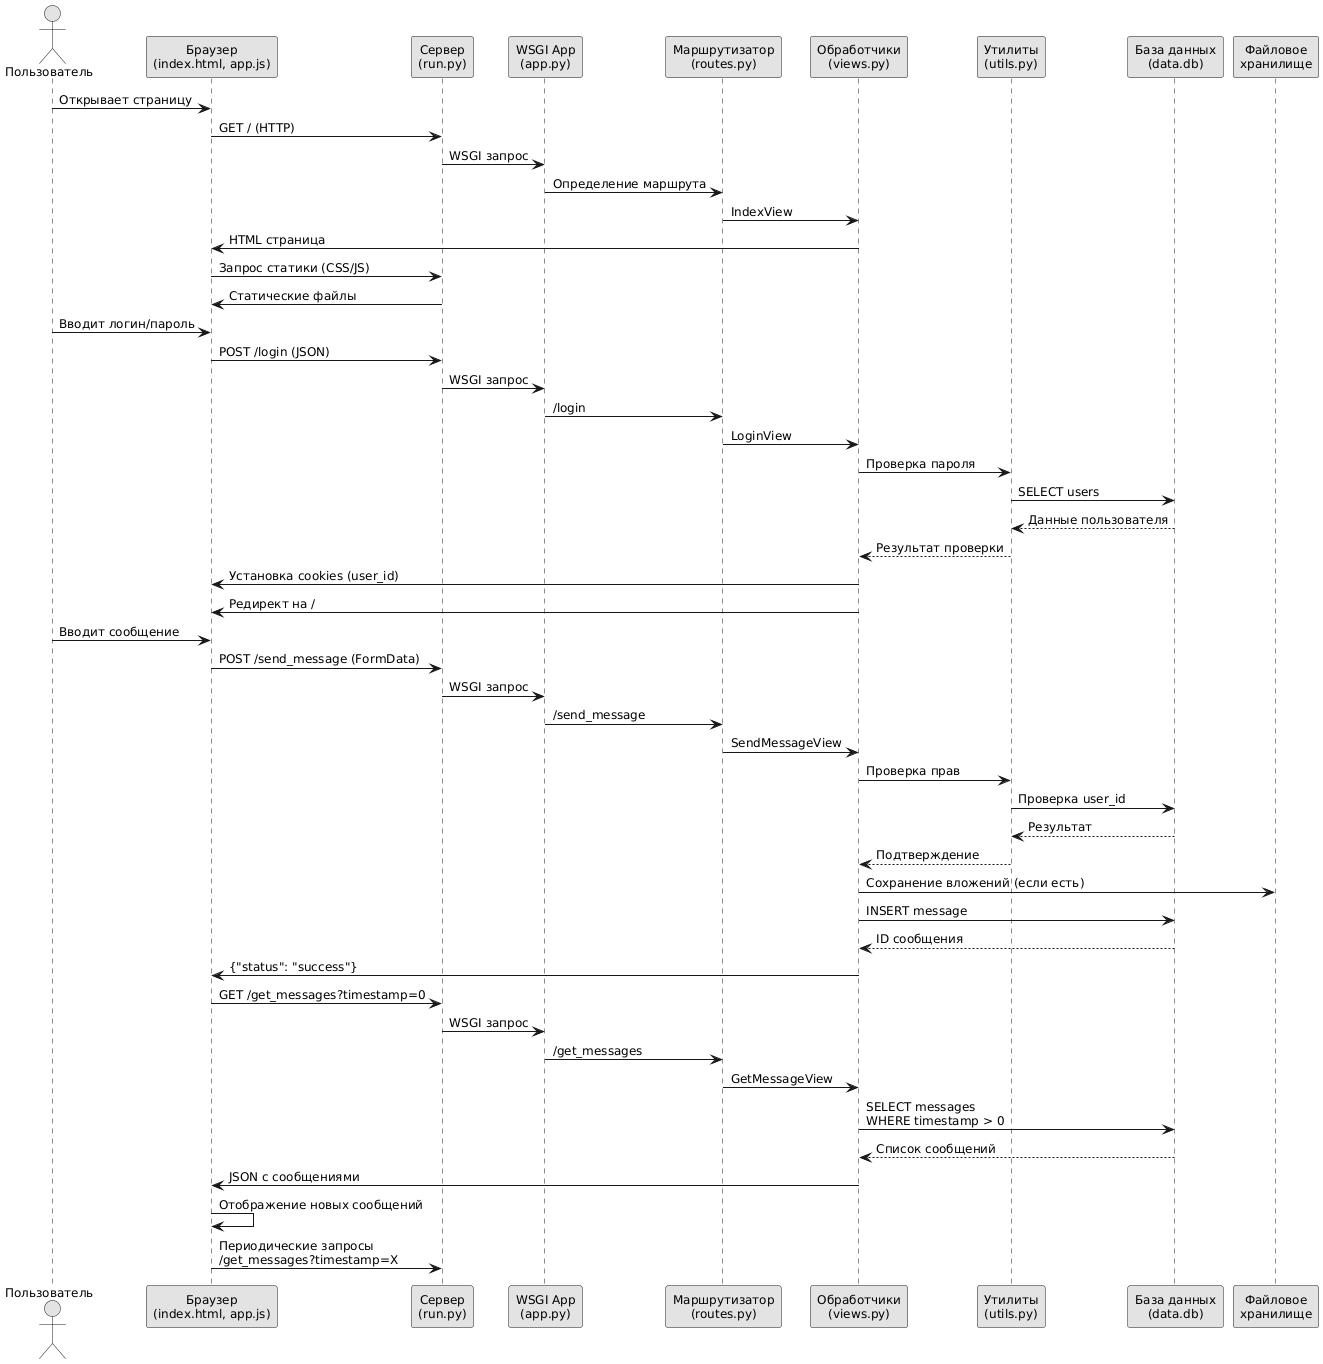
\includegraphics[width=1\linewidth]{Диаграмма последовательности}}
	\caption{Диаграмма компонентов}
	\label{data:image}
\end{figure}

\begin{enumerate}[leftmargin=*,label=\textbf{\arabic*.}]
	\item \textbf{Загрузка страницы (инициализация)}
	\begin{itemize}
		\item пользователь открывает в браузере главную страницу (index.html);
		\item браузер отправляет HTTP GET-запрос на сервер;
		\item серверный скрипт run.py (Waitress) получает запрос;
		\item запрос передаётся в WSGI-приложение (app.py);
		\item маршрутизатор (routes.py) определяет обработчик IndexView;
		\item пользователю возвращается HTML-страница и статические файлы (CSS/JS).
	\end{itemize}
	
	\item \textbf{Процесс аутентификации}
	\begin{itemize}
		\item пользователь вводит логин и пароль в форму входа;
		\item браузер отправляет POST /login запрос (JSON);
		\item LoginView проверяет учётные данные:
		\begin{itemize}
			\item через utils.py выполняется SQL-запрос к таблице users;
			\item пароль проверяется с помощью bcrypt.
		\end{itemize}
		\item при успешной аутентификации:
		\begin{itemize}
			\item устанавливается cookie с user\_id;
			\item происходит редирект на главную страницу.
		\end{itemize}
	\end{itemize}
	
	\item \textbf{Отправка нового сообщения}
	\begin{itemize}
		\item пользователь вводит текст и/или прикрепляет файлы;
		\item браузер формирует FormData и отправляет POST /send\_message;
		\item SendMessageView выполняет:
		\begin{itemize}
			\item проверку прав через cookies;
			\item сохранение файлов в static/uploads;
			\item запись сообщения в БД (таблицы messages или group\_messages);
		\end{itemize}
		\item клиент получает JSON с результатом операции;
	\end{itemize}
	
	\item \textbf{Получение сообщений (реализация чата)};
	\begin{itemize}
		\item браузер периодически опрашивает сервер (GET /get\_messages);
		\item GetMessageView запрашивает новые сообщения из БД;
		\item сервер возвращает JSON с массивом сообщений;
		\item браузер динамически обновляет интерфейс чата;
	\end{itemize}
	
	\item \textbf{Особенности работы}
	\begin{itemize}
		\item все запросы проходят через единую точку входа (app.py);
		\item маршрутизатор выбирает соответствующий View-класс;
		\item бизнес-логика сосредоточена во views;
		\item работа с БД вынесена в db\_utils.py;
		\item файлы хранятся локально в файловой системе;
		\item состояние сессии поддерживается через cookies.
	\end{itemize}
\end{enumerate}

\subsection{Диаграмма размещения}

Диаграмма размещения (рис.~\ref{place:image}) отражает физические взаимосвязи между программными и аппаратными компонентами системы.

\begin{figure}[ht]
\center{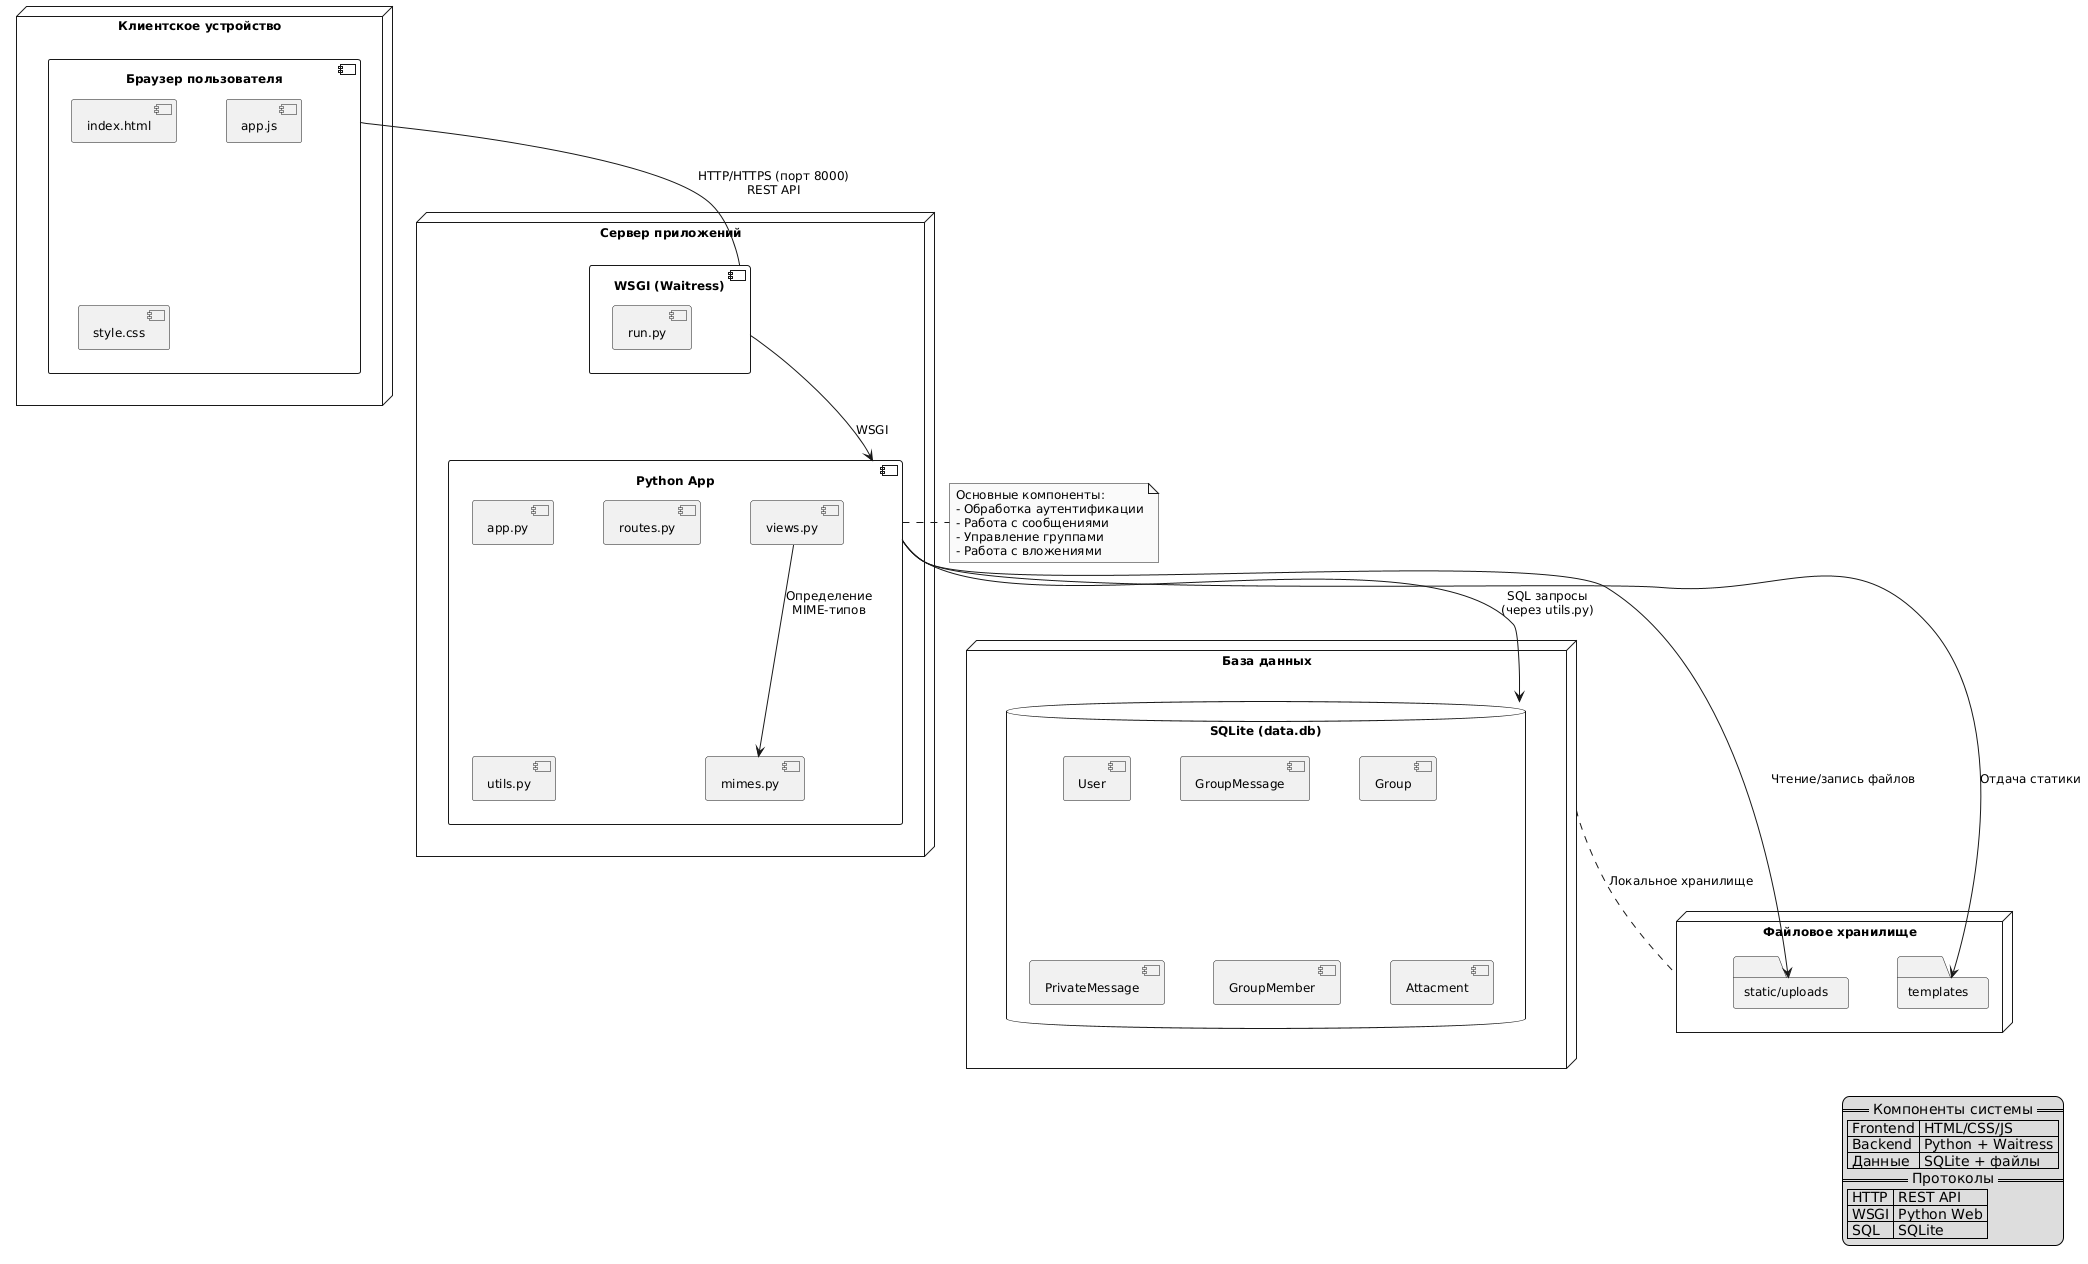
\includegraphics[width=1\linewidth]{Диаграмма развёртывания}}
\caption{Диаграмма развёртывания}
\label{place:image}
\end{figure}

Диаграмма развертывания отображает архитектуру корпоративного мессенджера. На стороне клиента взаимодействие с системой осуществляется через веб-браузер, который загружает статические файлы интерфейса — HTML-шаблоны, JavaScript-код и CSS-стили.

Серверная часть реализована на Python с использованием WSGI-сервера Waitress, обрабатывающего входящие HTTP-запросы на порту 8000. Логика приложения организована в виде пакетов views и models. Пакет views содержит специализированные модули для обработки запросов: auth.py отвечает за аутентификацию, groups.py управляет групповыми чатами, message.py обрабатывает сообщения, p\_chat.py обеспечивает личную переписку. Пакет models включает UserModel.py, GroupModel.py и MessageModel.py, инкапсулирующие работу с данными. Вспомогательные функции вынесены в utils.py и mimes.py.

Хранение данных организовано в двух форматах. Реляционная база SQLite (файл data.db) содержит таблицы User, Group, GroupMember, GroupMessage, PrivateMessage и Attachment, обеспечивающие хранение структурированной информации о пользователях, чатах, сообщениях и вложениях. Файловое хранилище в папках static/uploads и templates обслуживает медиафайлы и шаблоны интерфейса.

Взаимодействие между компонентами осуществляется через API между клиентом и сервером. WSGI-сервер передает запросы в Python-приложение, где они обрабатываются соответствующими модулями пакета views. Для работы с данными views используют методы пакета models, которые выполняют SQL-запросы к базе данных. Файловые вложения передаются напрямую через специальные обработчики.

Архитектура системы сохраняет принцип самодостаточности — все компоненты развертываются на едином сервере без внешних зависимостей. Четкое разделение на модули views и models обеспечивает безопасность и упрощает дальнейшее развитие системы, сохраняя при этом возможность автономной работы в корпоративной сети.

